\documentclass{tutorial}
\usepackage{tikz, tkz-berge, multirow}
\usetikzlibrary{arrows,%
                petri,%
                topaths}%
\begin{document}
\newif\ifsolns

%%%%%%%%%%%%%%%%%%%%%%%%%
% UNCOMMENT BELOW TO TURN ON SOLNS %
%%%%%%%%%%%%%%%%%%%%%%%%%
\solnstrue

\title{EE241 Spring 2015: Tutorial \#13}
\date{Friday, April 24, 2015}
\maketitle



\begin{prob}[Least squares]
Find the least squares fit of the equation $y = ax+b$ for the points $(1,2)$, $(2,2)$, $(3,2)$, and $(4,3)$. 
\end{prob} \ifsolns \begin{proof}
We can start with the exact fit equation of the form $X\vec{p} = Y$ where $X$ and $Y$ are our data and $\vec{p}$ are the parameters that fit them. The key is to treat the points enumerated above as the ``constraints'' and $a$ and $b$ as the variables we are solving for
\[
  X \vec{p} = Y
  \hspace{0.15in} \Longrightarrow \hspace{0.15in}
  \ls \begin{array}{rr}
    1 & 1 \\
    2 & 1 \\
    3 & 1 \\
    4 & 1
  \end{array} \rs
  \ls \begin{array}{r} a \\ b \end{array} \rs
  = \ls \begin{array}{r}
    2 \\ 2 \\ 2 \\ 3
  \end{array} \rs .
\]
Notice that we've added the column of $1$'s that correspond to the coefficients on the variable $b$. Of course, the matrix equation we've written above has no solution. However! The associated \emph{normal equations} do. We can get the normal equations by applying $X^T$ to both sides of the equations above
\[
  X^TX \vec{p} = XY
  \hspace{0.15in} \Longrightarrow \hspace{0.15in}
  \ls \begin{array}{rrrr}
    1 & 2 & 3 & 4 \\
    1 & 1 & 1 & 1
  \end{array} \rs
  \ls \begin{array}{rr}
    1 & 1 \\
    2 & 1 \\
    3 & 1 \\
    4 & 1
  \end{array} \rs
  \ls \begin{array}{r} a \\ b \end{array} \rs
  = \ls \begin{array}{rrrr}
    1 & 2 & 3 & 4 \\
    1 & 1 & 1 & 1
  \end{array} \rs \ls \begin{array}{r}
    2 \\ 2 \\ 2 \\ 3
  \end{array} \rs .  
\]
This reduces to
\[
  \ls \begin{array}{rr}
    30 & 10 \\
    10 & 4
  \end{array} \rs
  \ls \begin{array}{r} a \\ b \end{array} \rs
  = \ls \begin{array}{r}
    24 \\ 9
  \end{array} \rs 
\]
which has the solution $a = 0.3$, $b=1.5$.
\end{proof}\else \newpage \fi



\begin{prob}[Eigenvalues and eigenvectors practice]
Find the eigenvalues of the following matrices
\[
  (a) \;\; \ls \begin{array}{rrr}
     2 &  4 & -2 \\
     4 &  2 &  0 \\
    -2 &  0 &  2
  \end{array} \rs
  \hspace{0.15in}
  (b) \;\; \ls \begin{array}{rrrr}
     1 &  0 &  0 &  0 \\
     1 &  2 &  0 &  0 \\
     0 &  1 &  3 &  0 \\
     0 &  0 &  1 &  4
  \end{array} \rs
  \hspace{0.15in}
  (c) \;\; \ls \begin{array}{rr}
    0 & 1 \\ 0 & 0
  \end{array} \rs
\]
Find the eigenvectors of matrix (a). \textbf{Aside:} In general, we can define eigen\textbf{functions} as well as eigenvectors. The derivative operator ($d/dx$) on real-valued functions ($f(x): \mbR \rightarrow \mbR$) is a linear transformation. What functions are eigenfunctions of $d/dx$? What are their eigenvalues?
\end{prob} \ifsolns \begin{proof}
First, the eigenvalues
\begin{enumerate}[label=(\alph*)]
\item The characteristic equation is
\[
  \left| \begin{array}{rrr}
     2-\lambda &  4 & -2 \\
     4 &  2-\lambda &  0 \\
    -2 &  0 &  2-\lambda
  \end{array} \right| = 0
  \hspace{0.15in} \Longrightarrow \hspace{0.15in}
  (2-\lambda)^3 - 4 \lp 4(2-\lambda) \rp - 2 \lp 2(2-\lambda)\rp  = 0
\]
which means that
\begin{align*}
  0 &= (2-\lambda) \lp (2-\lambda)^2 - 16 - 4 \rp \\
  0 &= (2-\lambda) \lp 4 - 4\lambda + \lambda^2 - 20 \rp \\
  0 &= (2-\lambda) \lp \lambda^2 - 4 \lambda - 16 \rp
\end{align*}
Thus
\[
  \lambda = \lb \begin{array}{l}
    2, \\
    2+\sqrt{20}, \\
    2-\sqrt{20}
  \end{array} \right.
\]
\item In this case, the characteristic equation reduces much more quickly, consider
\[
  \left| \begin{array}{rrrr}
     1-\lambda &  0 &  0 &  0 \\
     1 &  2-\lambda &  0 &  0 \\
     0 &  1 &  3-\lambda &  0 \\
     0 &  0 &  1 &  4-\lambda
  \end{array} \right|
  \hspace{0.15in} \Longrightarrow \hspace{0.15in}
  (1-\lambda)(2-\lambda)(3-\lambda)(4-\lambda) = 0
\]
and so the eigenvalues are $\lambda = 1,2,3,4$.
\item In this case there is one eigenvalue repeated twice. The eigenvalues is $0$.
\end{enumerate}
To find the eigenvectors of matrix (a) We just need to solve for $\vec{v}$ in the three equations
\begin{align*}
  \lp A - 2 I_3 \rp \vec{v}_1 & = \vec{0} \\
  \lp A - (2+\sqrt{20}) I_3 \rp \vec{v}_2 & = \vec{0} \\
  \lp A - (2-\sqrt{20}) I_3 \rp \vec{v}_3 & = \vec{0} .
\end{align*}
The three vectors (solved using MATLAB) are
\begin{align*}
  \vec{v}_1 & = \ls 0 \; , \; 0.4472 \; , \; 0.8944 \rs \\
  \vec{v}_2 & = \ls 0.7071 \;, \; -0.6325 \; , \; 0.3162 \rs \\
  \vec{v}_3 & = \ls -0.7071 \;, \; -0.6325 \; , \; 0.3162 \rs .
\end{align*}
As to the ``aside'' question on eigenfunctions, notice that
\[
  \frac{d}{dx} f(x) = \lambda f(x)
\]
for $f(x) = e^{\lambda x}$. Thus the exponential function for \emph{any} coefficient $\lambda$ is an eigenfunction of the derivative operator with eigenvalue $\lambda$.
\end{proof}\else \newpage \fi



\begin{prob}[Diagonalizing a matrix]
Pick the diagonalizeable matrix below and find $A = P D P^T$ where $D$ is diagonal and $P$ is orthonormal.
\[
  (a) \ls \begin{array}{rrr}
    1 & 0 & 0 \\
    1 & 2 & 0 \\
    1 & 2 & 3
  \end{array} \rs
  \hspace{0.15in}
  (b) \ls \begin{array}{rrr}
    1 & 2 & 2 \\
    2 & 3 & 3 \\
    2 & 3 & 3
  \end{array} \rs
  \hspace{0.15in}
  (c) \ls \begin{array}{rrr}
    1 &-1 &-1 \\
    1 & 2 &-2 \\
    1 & 2 & 3    
  \end{array} \rs
\]
\end{prob} \ifsolns \begin{proof}
In the above, only matrix (b) is symmetric and so can be diagonalized. To compute $D$ we need the eigenvalues, to compute $P$ we need the eigenvectors. The characteristic equation is
\[
  \left| \begin{array}{rrr}
    1-\lambda & 2 & 2 \\
    2 & 3-\lambda & 3 \\
    2 & 3 & 3-\lambda
  \end{array} \right|
  \hspace{0.15in} \Longrightarrow \hspace{0.15in}
  (1-\lambda) \lp (3-\lambda)^2 - 9 \rp - 2 \lp 2(3-\lambda) - 6 \rp + 2 \lp 6 - 2 (3-\lambda) \rp = 0
\]
Solving,
\begin{align*}
  0 &= (1-\lambda) \lp (3-\lambda)^2 - 9 \rp - 4 \lp 2(3-\lambda) - 6 \rp \\
  0 &= (1-\lambda) \lp (3-\lambda)^2 - 9 \rp - 4 \lp -2\lambda \rp \\
  0 &= (1-\lambda) \lp - 6\lambda + \lambda^2 \rp +8 \lambda \\
  0 &= \lambda \lp (1-\lambda)(-6+\lambda) + 8 \rp \\
  0 &= \lambda \lp -\lambda^2 + 7 \lambda +2\rp
\end{align*}
and the eigenvalues are $\lambda_1 = 0$ $\lambda_2 = (7+\sqrt{57})/2$ $\lambda_3 = (7-\sqrt{57})/2$. The eigenvectors come from solving the characteristic equation with each $\lambda$ substituted in. That is,
\begin{align*}
  A \vec{v}_1 & = \vec{0} \\
  \lp A - (7+\sqrt{57})/2 I_3 \rp \vec{v}_2 & = \vec{0} \\
  \lp A - (7-\sqrt{57})/2 I_3 \rp \vec{v}_3 & = \vec{0} .
\end{align*}
Note that $\vec{v}_1$ is simply the normalized vector that defines the nullspace of $A$. The three vectors are
\begin{align*}
  \vec{v}_1 & = \ls 0 \; , \; 1/\sqrt{2}\; , \; -1/\sqrt{2} \rs \\
  \vec{v}_2 & = \ls 0.4109 \;, \; 0.6446 \; , \; 0.6446 \rs \\
  \vec{v}_3 & = \ls 0.9117 \;, \; -0.2906 \; , \; -0.2906 \rs .
\end{align*}
\end{proof}\else \newpage \fi



\begin{prob}[Adjacency matrices for social networks]
Recall that for a graph $G$ the adjacency matrix is given by
\[
  \ls A_G \rs_{ij} = \lb \begin{array}{lcl}
    1 & \hspace{0.15in} & i,j \; \text{connected} \\
    0 & & \text{otherwise}
  \end{array} \right. 
\]
(assume no self-loops). We'll now also add to these definitions, the \emph{degree matrix} $D_G$ which is defined as
\[
  \ls D_G \rs_{ij} = \lb \begin{array}{lcl}
    d_i & \hspace{0.15in} & i=j \\
    0 & & \text{otherwise}
  \end{array} \right.
\]
where $d_i$ is the number of connections at node $i$. Finally, if we take the difference of these two matrices we get the \emph{graph Laplacian} $L_G$,
\[
  L_G = D_G - A_G
\]
The number of times $0$ appears as an eigenvalue in the Laplacian is the number of connected components in the graph. Connected components are like ``islands'' in social networks, it is impossible to be introduced to someone on another island via mutual friends. How many $0$ eigenvalues are there in the following matrix?
\[
  L_G = \ls \begin{array}{rrrrrr}
     2 & -1 & -1 &  0 &  0 &  0 \\
    -1 &  3 & -1 & -1 &  0 &  0 \\
    -1 & -1 &  3 & -1 &  0 &  0 \\
     0 & -1 & -1 &  2 &  0 &  0 \\
     0 &  0 &  0 &  0 &  1 & -1 \\
     0 &  0 &  0 &  0 & -1 &  1
  \end{array} \rs
\]
Sketch the graph it represents. What fundamental matrix quantity does the number of $0$ eigenvalues correspond to?
\end{prob} \ifsolns \begin{proof}
In the matrix $L_G$ there are two connected components and therefore there are two $0$ eigenvalues. We can check this fact by putting the matrix in MatLAB to get the eigenvalues (via the \textsc{eig} function)
\[
  \lambda = 0,0,2,2,4,4 .
\]
The graph associated with this matrix can be easily drawn by looking at the off-diagonal elements of $L_G$ since they correspond to $A_G$,
\begin{center} 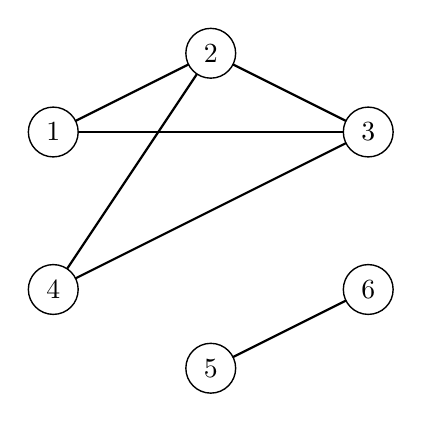
\begin{tikzpicture}[scale=1,transform shape]
  \Vertex[x= 2,y= 3] 1
  \Vertex[x= 4,y= 4] 2 
  \Vertex[x= 6,y= 3] 3 
  \Vertex[x= 2,y= 1] 4
  \Vertex[x= 4,y= 0] 5
  \Vertex[x= 6,y= 1] 6
  \Edge (1)(2)
  \Edge (1)(3)
  \Edge (2)(3)
  \Edge (2)(4)
  \Edge (3)(4)
  \Edge (5)(6)
\end{tikzpicture} \end{center}
The fundamental matrix quantity related to the number of $0$ eigenvalues (and indeed, the number of connected components of the associated graph) is the \emph{dimension of the nullspace}. Indeed, by using the \textsc{null} function in MatLab we get two linearly independent vectors
\[
  \vec{v}_1 = \ls 1/2, 1/2, 1/2, 1/2, 0, 0 \rs
  \hspace{0.15in} \text{and} \hspace{0.15in}
  \vec{v}_2 = \ls 0, 0, 0, 0, 1/\sqrt{2}, 1/\sqrt{2} \rs .
\]
\end{proof}\else \newpage \fi

\end{document}













